\documentclass{beamer} % imports amsmath symbols

\usepackage{mathleague}

\newcommand{\contestproblemset}{12117}
\newcommand{\roundname}{Target}
\newcommand{\problemnumber}{4}

\begin{document}

\begin{frame} % Title Page
  \titlepage
\end{frame}

\section{Problem}

\subsection*{Identify the objective.}

\begin{frame}
  An equiangular but not equilateral hexagon has three times the area of a regular hexagon with side length $1$. If both hexagons have whole number side lengths, then what is the perimeter of the larger hexagon?
\end{frame}

\section{Solution}

\subsection*{Find the perimeter of an equiangular (non-equilateral) hexagon that has thrice the area of a regular hexagon with side length \texorpdfstring{$1$}{1}.}

\begin{frame}
  \begin{center}
    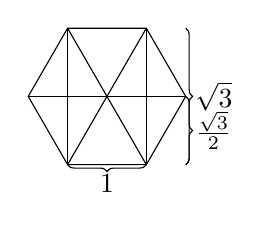
\begin{tikzpicture}
      \draw (0,0) -- (-0.5,0.866025404) -- (0,1.73205081) -- (1,1.73205081) -- (1.5,0.866025404) -- (1,0) -- cycle;
      \draw [decoration={brace,mirror,raise=0.0cm},decorate] (0,0) -- (1,0) node [midway,below=0.0cm] {$1$};
      \draw<3-6> (0,0) -- (0.5,0.866025404);
      \draw<3-6> (-0.5,0.866025404) -- (0.5,0.866025404);
      \draw<3-6> (0,1.73205081) -- (0.5,0.866025404);
      \draw<3-6> (1,1.73205081) -- (0.5,0.866025404);
      \draw<3-6> (1.5,0.866025404) -- (0.5,0.866025404);
      \draw<3-6> (1,0) -- (0.5,0.866025404);
      \draw<4-6> [decoration={brace,mirror,raise=0.5cm},decorate] (1,0) -- (1,0.866025404) node [midway,right=0.5cm] {$\frac{\sqrt{3}}{2}$};
      \draw<7-> (0,0) -- (0,1.73205081);
      \draw<7-> (1,0) -- (1,1.73205081);
      \draw<7-> [decoration={brace,mirror,raise=0.5cm},decorate] (1,0) -- (1,1.73205081) node [midway,right=0.5cm] {$\sqrt{3}$};
    \end{tikzpicture}
  \end{center}

  \uncover<2->{$\text{Area} \only<4-5>{= 6 \cdot \frac{1}{2} \cdot 1 \cdot \frac{\sqrt{3}}{2}} \uncover<5->{= \frac{3}{2} \cdot \sqrt{3}} \uncover<7->{\text{, so we need an additional } 3 \cdot \sqrt{3}.}$}

  \begin{center}
    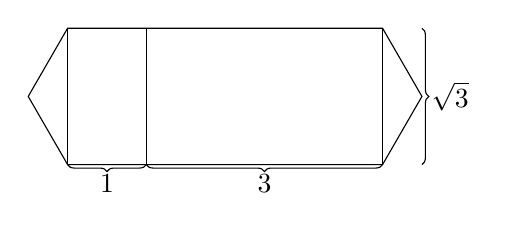
\begin{tikzpicture}
      \draw<8-> (0,0) -- (-0.5,0.866025404) -- (0,1.73205081) -- (4,1.73205081) -- (4.5,0.866025404) -- (4,0) -- cycle;
      \draw<8-> (0,0) -- (0,1.73205081);
      \draw<8-> (1,0) -- (1,1.73205081);
      \draw<8-> (4,0) -- (4,1.73205081);
      \draw<8-> [decoration={brace,mirror,raise=0.5cm},decorate] (4,0) -- (4,1.73205081) node [midway,right=0.5cm] {$\sqrt{3}$};
      \draw<8-> [decoration={brace,mirror,raise=0.0cm},decorate] (0,0) -- (1,0) node [midway,below=0.0cm] {$1$};
      \draw<8-> [decoration={brace,mirror,raise=0.0cm},decorate] (1,0) -- (4,0) node [midway,below=0.0cm] {$3$};
    \end{tikzpicture}
  \end{center}

  \uncover<9->{$\text{Area} = \frac{3}{2} \cdot \sqrt{3} + 3 \cdot \sqrt{3} = \frac{9}{2} \cdot \sqrt{3}\uncover<10->{, \text{Perimeter} = 2 \cdot 4 + 4 \cdot 1 = \boxed{12}}$}
\end{frame}

\setcounter{equation}{0} % Place this after each frame that uses equations to reset the counter

\section{Reflection}

\subsection*{Review the concepts.}

\begin{frame}
  \frametitle{Concepts}
  \begin{itemize}
    \item area of an equilateral triangle
    \item<2-> area of a rectangle
    \item<3-> area of a regular hexagon
  \end{itemize}
\end{frame}

\end{document}